\documentclass[10pt,a4paper]{article}
\usepackage{amsmath}
% \usepackage[margin=1in]{geometry}
\usepackage[a4paper,top=1in, bottom=1in, left=1in, right=1in]{geometry}
\usepackage{amsmath}
\usepackage{amssymb}
\usepackage{color}
\usepackage{graphicx}
\usepackage{fancyhdr}
\usepackage{url}
\usepackage[spanish]{babel}% Lenguage-specific commands
%\usepackage[english]{babel}
\usepackage[utf8x]{inputenc} % is no longer required (since 2018)
\usepackage[T1]{fontenc}% Set the font (output) encodings
%%%%%%%%%%%%%%%%%%%%%%%%%%%%%%%%%%%%%%%%%%%%%%%%%%%%%%
% lstlisting
%%%%%%%%%%%%%%%%%%%%%%%%%%%%%%%%%%%%%%%%%%%%%%%%%%%%%%
\usepackage{listings}             % Include the listings-package
\usepackage{alltt}
\definecolor{codegreen}{rgb}{0,0.6,0}
\definecolor{codegray}{rgb}{0.5,0.5,0.5}
\definecolor{codepurple}{rgb}{0.58,0,0.82}
\definecolor{backcolour}{rgb}{0.95,0.95,0.92}

\lstdefinestyle{mystyle}{
    backgroundcolor=\color{backcolour},
    commentstyle=\color{codegreen},
    keywordstyle=\color{codepurple},
    numberstyle=\tiny\color{codegray},
    stringstyle=\color{codepurple},
    basicstyle=\ttfamily\small,
    breakatwhitespace=false,
    breaklines=true,
    captionpos=b,
    keepspaces=true,
    numbers=left,
    numbersep=5pt,
    showspaces=false,
    showstringspaces=false,
    showtabs=false,
    tabsize=2,
    language=Fortran
}

\lstset{style=mystyle}

%%%%%%%%%%%%%%%%%%%%%%%%%%%%%%%%%%%%%%%%%%%%%%%%%%%%%%
% Graphs path to the Picture Folder
%%%%%%%%%%%%%%%%%%%%%%%%%%%%%%%%%%%%%%%%%%%%%%%%%%%%%%
\graphicspath{{Pictures/}{Data/}} % Two folders Picture and Data


\newcommand{\myUniversidad}{Universidad Nacional del Callao}
\newcommand{\myFacultad}{Facultad de Ingenier\'ia Mec\'anica y de Energ\'ia}
% \newcommand{\myEscuelaProfesional}{ESCUELA PROFESIONAL DE F\'ISICA}
\newcommand{\myCurso}{Laboratorio de F\'isica I}
\newcommand{\myTarea }{Nombre de la Experiencia - Laboratorio }
\newcommand{\myNombre}{Apellidos y Nombres}
% \newcommand{\myEmail}{email\_name@unac.gob.pe}
\newcommand{\myNumTarea}{5} % Cambie el numero de Laboratorio

\pagestyle{fancyplain}
\lhead{\fancyplain{}{\textbf{Laboratorio \myNumTarea}}}      
\rhead{\fancyplain{}{\myNombre}}

%%%%%%%%%%%%%%%%%%%%%%%%%%%%%%%%%%%%%%%%%%%%%%%%%%%%%%
% bibliography
%%%%%%%%%%%%%%%%%%%%%%%%%%%%%%%%%%%%%%%%%%%%%%%%%%%%%%
%\usepackage{biblatex}
\bibliographystyle{plain}

%%%%%%%%%%%%%%%%%%%%%%%%%%%%%%%%%%%%%%%%%%%%%%%%%%%%%%
% Begin Document
%%%%%%%%%%%%%%%%%%%%%%%%%%%%%%%%%%%%%%%%%%%%%%%%%%%%%%
\begin{document}
%--------------------------------------------------------------------------------------------------
\thispagestyle{plain} % plain permite que la primera pagina no aparescan la barra en la parte superior de la pagina
%--------------------------------------------------------------------------------------------------
\begin{minipage}{.30\textwidth}
 
\includegraphics[width=.5\textwidth]{Escudo_UNAC.png}\\[.5cm]
\end{minipage}
\begin{minipage}{.65\textwidth}
\begin{center} 
\Large{                
\myUniversidad\\
\myFacultad\\ 
\myCurso\\
{\myTarea \myNumTarea}\\
\myNombre\\
\today}
\end{center} 
\end{minipage}\\
%--------------------------------------------------------------------------------------------------
\centerline{\underline{\hspace{7in}}}
%--------------------------------------------------------------------------------------------------
\tableofcontents
%--------------------------------------------------------------------------------------------------


\section{Contenido / Marco teórico:} 

Expone de manera clara y sintética los conceptos teóricos que sustentan los objetivos planteados, así como aquellos en los que se basa la experiencia práctica realizada  \cite{Ding_and_Williams, Ling2016v1, Ling2016v2, Ling2016v3}.  

\section{Análisis de datos:} 

Presenta de forma clara, sintética y crítica ecuaciones, gráficos, diagramas o figuras que evidencian la problemática analizada. Incluye el manejo de incertidumbres y un adecuado procesamiento de datos e información \cite{Yang_Kurth_Willians, Young2012v1, Young2012v2}.  
\begin{equation}
  x_{n+1}  =  x_n - m\;f(x)\left[\frac{x_n-x_{n-1}}{f(x_n)-f(x_{n-1}}\right]
\end{equation}
\hspace{1mm}\\
For $m=\frac{1+\sqrt{5}}{2}=1.618$\\
\begin{verbatim}
Steps        xa              xb               xi           f(xi)       |(xn+1-xn)|
----------------------------------------------------------------------------------
  0  1.500000000000  1.600000000000  1.633191538329 -0.001945949763  0.033191538329 
  1  1.600000000000  1.633191538329  1.564416498720 -0.000020351034  0.068775039609 
  2  1.633191538329  1.564416498720  1.563240412447 -0.000028545785  0.001176086273 
  3  1.564416498720  1.563240412447  1.569869184045 -0.000000429797  0.006628771598 
  4  1.563240412447  1.569869184045  1.570033141259 -0.000000291226  0.000163957214 
  5  1.569869184045  1.570033141259  1.570590682342 -0.000000021145  0.000557541083 
  6  1.570033141259  1.570590682342  1.570661309883 -0.000000009115  0.000070627541 
  7  1.570590682342  1.570661309883  1.570747894571 -0.000000001173  0.000086584688 
  8  1.570661309883  1.570747894571  1.570768583633 -0.000000000385  0.000020689062 
  9  1.570747894571  1.570768583633  1.570784932394 -0.000000000065  0.000016348761 
 10  1.570768583633  1.570784932394  1.570790299953 -0.000000000018  0.000005367559 
 11  1.570784932394  1.570790299953  1.570793673498 -0.000000000004  0.000003373545 
 12  1.570790299953  1.570793673498  1.570794985787 -0.000000000001  0.000001312289 
 13  1.570793673498  1.570794985787  1.570795714281 -0.000000000000  0.000000728494 
\end{verbatim}
\begin{lstlisting}
! Codigo Fortran aqui
PROGRAM ejemplo
  IMPLICIT NONE
  INTEGER :: i, n
  REAL :: x, sum

  n = 100
  sum = 0.0

  DO i = 1, n
    x = REAL(i)
    sum = sum + x**2
  END DO

  PRINT *, 'La suma de los cuadrados es: ', sum

END PROGRAM ejemplo
\end{lstlisting}

\section{Resultados:} 

Organiza y presenta los datos obtenidos en párrafos, cuadros o gráficos debidamente identificados. Incorpora evidencia con imágenes rotuladas, relacionándolas con los resultados. Incluye las fórmulas y sustituciones utilizadas.  
% Puedes incluir una figura si es necesario
\begin{figure}[ht]
\centering
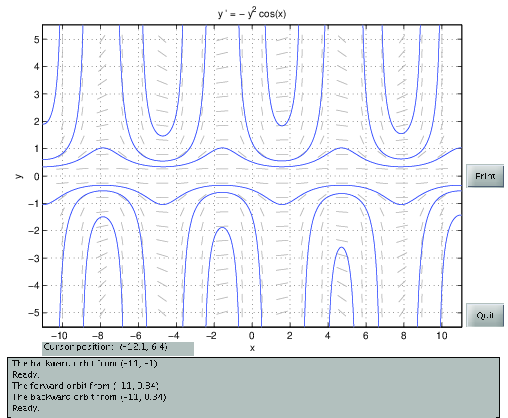
\includegraphics[width=0.5\textwidth]{fig1.png}
\caption{Diagrama esquemático del problema.}
\end{figure}

\begin{figure}[h]
    \centering
    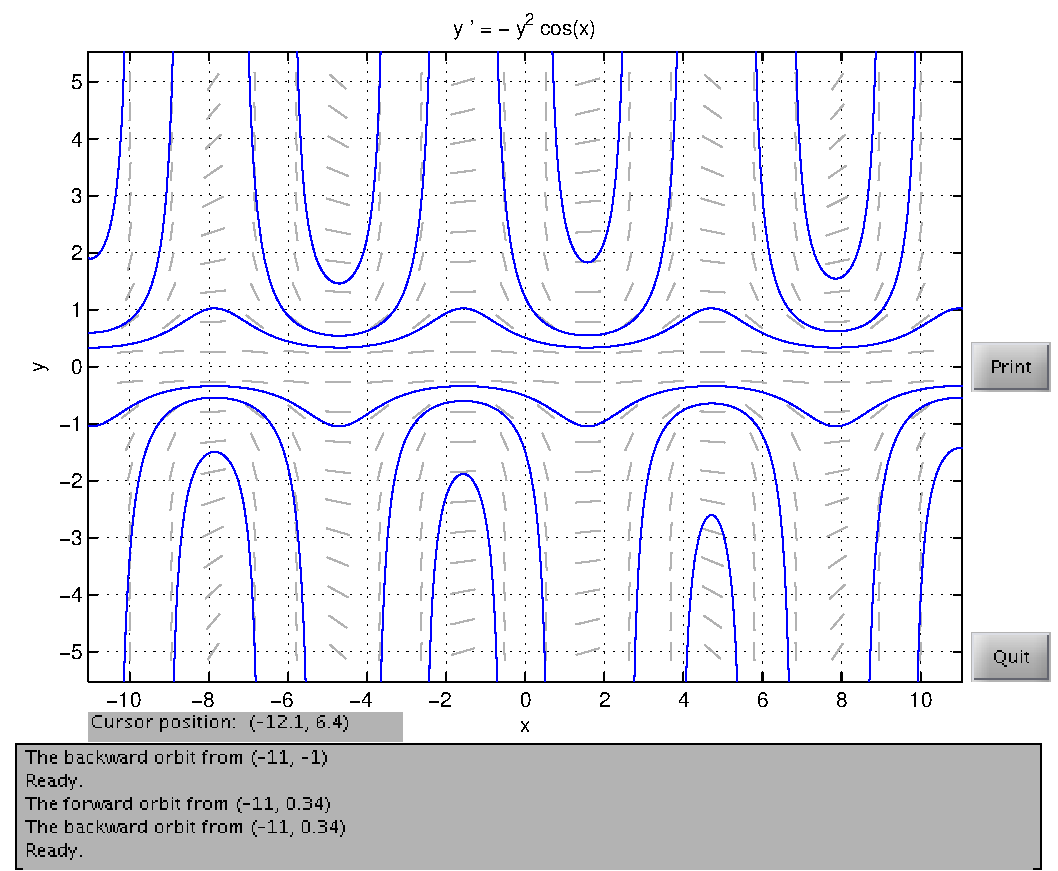
\includegraphics[width=0.5\textwidth]{fig2.pdf}
    \caption{Descripción de la figura}
\end{figure}

\section{Conclusiones / Discusión:} 

Formula conclusiones coherentes con los objetivos y la problemática planteada. Interpreta los resultados obtenidos, comparándolos con la bibliografía consultada, e indica posibles aplicaciones teóricas.  


%%%%%%%%%%%%%%%%%%%%%%%%%%%%%%%%%%%%%%%%%%%%%%%%%%%%%%%%%%%%%%%%%%%%%%%%%%%%%%%%
%                  Bibliography  or References page                            %                    
%%%%%%%%%%%%%%%%%%%%%%%%%%%%%%%%%%%%%%%%%%%%%%%%%%%%%%%%%%%%%%%%%%%%%%%%%%%%%%%%   
\addcontentsline{toc}{section}{References}
\bibliography{References/myBibliography}
\end{document}
